% ===========================================================================
% CAPÍTULO 4 — DISEÑO HARDWARE Y BANCO DE VALIDACIÓN
% ===========================================================================

Una vez completado el firmware del transceptor serie, se desarrolló el hardware de prueba
necesario para validar el sistema en condiciones reales. El plan inicial era diseñar una única
placa de comunicación serie para ejercitar múltiples líneas a la vez. Posteriormente, el proyecto
LINCE requirió dos tarjetas adicionales con especificaciones impuestas por Indra: la placa CDHS y
la placa AOCS. Estas placas permitieron a Indra validar su firmware sobre la ZCU102. Los
esquemáticos (PDF)
y las BOM de las tres placas están disponibles en el repositorio del proyecto~\cite{repo_tfm} bajo
\texttt{tfm/00\_docs/pcbs/}.

\section{Selección de componentes bajo la restricción de 1,8~V} \label{sec:seleccion_componentes}

La selección de componentes de las tres placas está condicionada por un límite eléctrico de la
plataforma.

Los bancos de entrada/salida del conector FMC HPC empleados por estas tarjetas operan a
\textbf{1,8~V}: es el nivel del carril \texttt{VADJ} con el que la ZCU102 alimenta la interfaz. Todo
componente que se conecte directamente a esos pines debe, por tanto, admitir una
\textit{VIO} (voltaje de bus) de 1,8~V. La \textit{VIO} es la tensión con la que se alimenta el
banco de entrada/salida digital de un circuito integrado, independiente de la de su núcleo. Fija
los niveles lógicos que la pieza acepta y entrega en sus pines. La alternativa, interponer
adaptadores de nivel entre el MPSoC y cada transceptor, añade componentes activos en el camino de
señal. Introduce además retardo de propagación en líneas que conmutan a varios megabaudios, y
multiplica los puntos de fallo. Se descartó salvo donde fue inevitable, y se buscaron
deliberadamente componentes con \textit{VIO} nativo a 1,8~V.

El criterio de partida no fue la cualificación formal para espacio. El componente cualificado es
la pieza \textit{rad-hard}, con un coste unitario y unos plazos de suministro que no encajan en un
programa NewSpace como LINCE. La práctica habitual en este ámbito es otra: emplear componentes de
catálogo, no cualificados oficialmente, que acreditan \textbf{herencia de vuelo} por haberse
utilizado ya en misiones anteriores.

La búsqueda se orientó por tanto a piezas de catálogo con herencia de vuelo, y no dio resultado.
Los transceptores de bus que la acreditan pertenecen a una generación tecnológica anterior y su
interfaz digital opera a 3,3~V o 5~V. No se encontró ninguno que admitiese una \textit{VIO} de 1,8~V,
de modo que la herencia de vuelo y el nivel de la plataforma resultaron incompatibles.

Al no encontrarse componentes con herencia de vuelo, se buscó el \textbf{grado automotriz} (cualificación
AEC-Q100\footnote{Norma del \textit{Automotive Electronics Council} que somete a los circuitos
integrados a ensayos de estrés (ciclado térmico, humedad, vida acelerada) para garantizar su
operación en el rango de temperatura y fiabilidad exigidos por la industria del automóvil.}).
Esta cualificación impone rangos de temperatura extendidos y niveles de robustez muy superiores a
los de grado comercial. Es el escalón al que se recurre en misiones de bajo coste cuando no hay
una pieza de catálogo con herencia de vuelo que cumpla los requisitos eléctricos. Los transceptores
\texttt{TCAN1044AVDRQ1} del bus CAN y el conversor analógico-digital \texttt{ADS7950QDBTRQ1} de la
placa CDHS responden a este criterio. Lo mismo ocurre con el transceptor \texttt{THVD1424RGTR} de
los canales serie de las placas CDHS y AOCS, elegido por soportar \textit{VIO} de 1,8~V de forma
nativa.

A estas tarjetas se les exige la \textbf{validación funcional} del subsistema de comunicaciones,
no ser un \textbf{modelo de vuelo}. El grado automotriz permitió ejercitar el subsistema en
condiciones eléctricas realistas dentro del coste y del plazo del trabajo.

La búsqueda deja además un dato aprovechable para el modelo de vuelo. Ningún transceptor de
catálogo con herencia de vuelo opera su interfaz digital a 1,8~V. Ese modelo tendrá que renunciar
al nivel nativo de la plataforma y adaptar la interfaz a piezas de 3,3~V o 5~V. Para ello, deberá
cambiar la tensión del carril \texttt{VADJ} o interponer adaptadores de nivel.

\section{Reglas de diseño y proceso de fabricación}

Las tres placas se diseñaron en \textbf{Altium Designer}. En los tres proyectos el primer paso,
antes de colocar ningún componente, fue definir las \textbf{reglas de diseño}. Altium las
comprueba de forma continua mientras se rutan las pistas. Definirlas al principio hace que una
restricción de fabricación incumplida salte como error en ese momento, y no como un rechazo del
fabricante con el diseño ya cerrado.

El criterio adoptado fue ceñirse a las \textbf{capacidades del proceso de fabricación del fabricante
seleccionado}, PCBWay~\cite{pcbway_caps}, en lugar de definir un conjunto de reglas propio. Los
límites de su proceso estándar (anchuras y separaciones mínimas de pista, diámetro mínimo de
taladro, anillo de vía y distancia mínima al borde de placa) son los que acotan lo que es
fabricable a coste ordinario. Apurarlos por debajo obliga a recurrir a procesos de precisión más
caros, y mantenerse muy por encima de ellos no aporta ninguna ventaja. Diseñar directamente contra esas
capacidades garantiza que las tres placas fueran fabricables en la primera tirada, como en efecto
ocurrió.

Sobre esas reglas generales se impusieron dos restricciones adicionales propias de las señales que
transportan estas placas. La primera es el \textbf{rutado en par diferencial} con impedancia
controlada para las líneas SPW, RS422/RS485 y CAN. La segunda es la
\textbf{longitud acotada} en las líneas de conmutación rápida procedentes del FMC, de manera que 
las señales tarden lo mismo en llegar a su destino.

\section{Diseño de la placa de comunicación serie} \label{sec:diseno_pcb_serie}

El objetivo de esta placa era poder ejercitar simultáneamente los 14 transceptores del IP core,
replicando las topologías de bus reales que se encontrarán en el satélite. Estas son RS485
multipunto, con múltiples nodos en el mismo cable, y RS422 en configuración \textit{master/slave},
con cruce de TX y RX. A diferencia de las placas CDHS y AOCS, cuyas especificaciones vinieron dictadas
por Indra, esta placa fue diseñada con total libertad para maximizar la flexibilidad de los
ensayos en laboratorio.

El transceptor seleccionado para los catorce canales es el \textbf{LTC2865}~\cite{ltc2865} de
Analog Devices, un transceptor RS485/RS422 de hasta 20~Mbps. Su pin de alimentación lógica
independiente (\texttt{VL}) le permite operar la interfaz digital directamente a los 1,8~V del
FMC, tal como exige la sección~\ref{sec:seleccion_componentes}. Expone además un
pin \texttt{SLO} de limitación de \textit{slew} controlable desde el MPSoC, que tendrá un papel
protagonista en la caracterización de la placa (sección~\ref{sec:pcb_slo}). Todas las líneas
diferenciales incorporan diodos TVS \textbf{SM712-02HTG} contra transitorios. Cada driver
dispone además de una resistencia de terminación de 120~$\Omega$ conmutable mediante
\textit{jumper}, lo que permite terminar el bus en los nodos extremos y dejar abiertos los
intermedios.

La arquitectura general de la placa divide los 14 canales en dos grupos conectados al FMC:

\begin{itemize}
    \item \textbf{7 drivers RS485 (RS0--RS6)} conectados a un bus diferencial común mediante
    \textit{jumpers}, formando una topología multipunto configurable.
    \item \textbf{7 drivers RS422 (RS7--RS13)} organizados en dos buses \textit{master/slave}
    independientes (BUS 1: 1 \textit{master} + 3 \textit{slaves}; BUS 2: 1 \textit{master} + 2 \textit{slaves}), con la línea
    TX cruzada con RX para emular la conexión real punto a punto RS422.
\end{itemize}

La hoja de nivel superior del esquemático (figura~\ref{fig:placa_serial_top}) recoge esta
arquitectura: el conector FMC en el centro, el bus común RS485 (RS0--RS6) a un lado y los dos
buses \textit{master/slave} RS422 (RS7--RS13) al otro. Cada bus sale por sus propios conectores
Dupont y Micro-D. El resultado físico del diseño se aprecia en el render de la
figura~\ref{fig:serial_3d}.

% Apaisada y a página completa a propósito: es la hoja más densa de las cinco y
% el tribunal puede leerla en papel, donde no se puede ampliar. Girada gana un
% 40 % de tamaño lineal frente a ponerla derecha al ancho de caja.
\begin{sidewaysfigure}
    \centering
    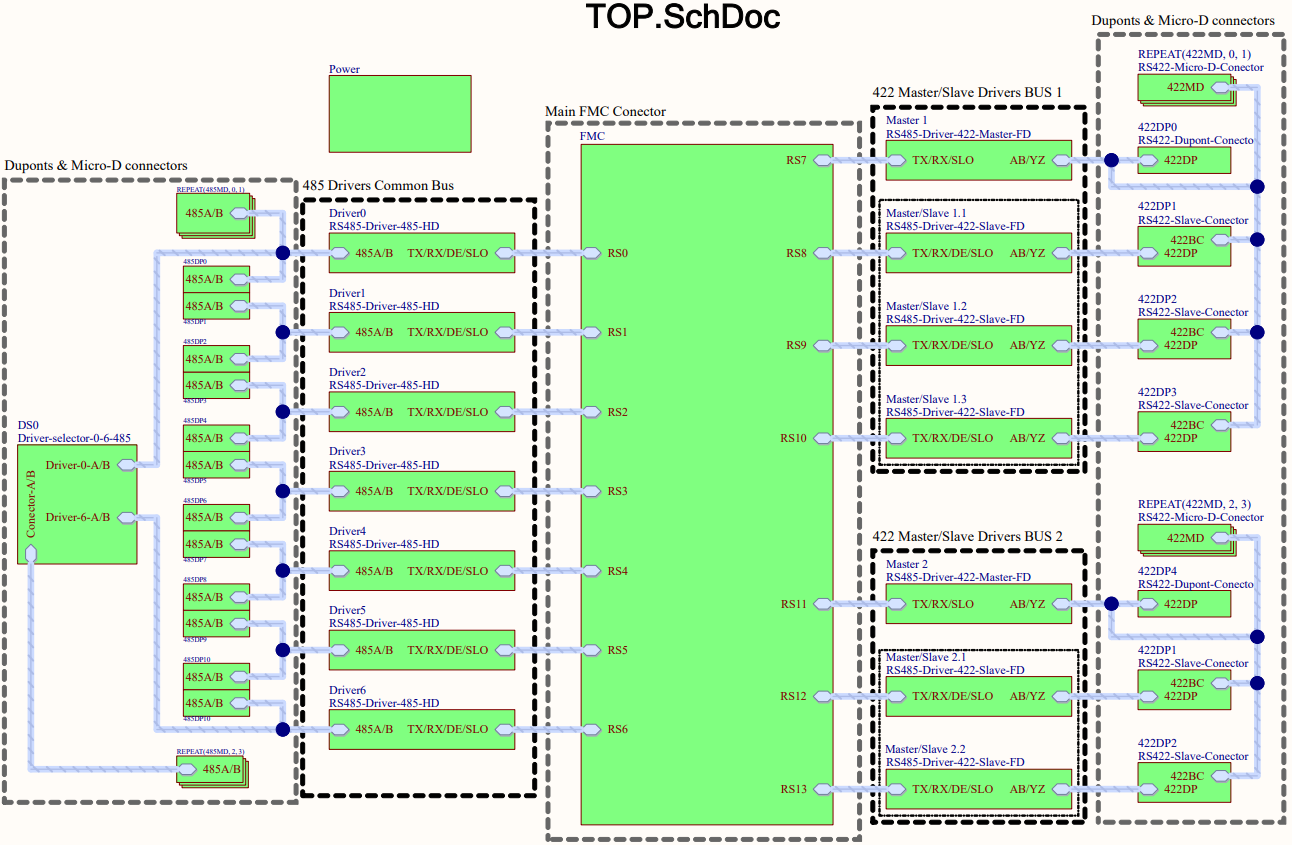
\includegraphics[width=0.95\textheight]{IMG/Esquematicos/serie.png}
    \caption{Hoja de nivel superior del esquemático de la placa de comunicación serie.}
    \label{fig:placa_serial_top}
\end{sidewaysfigure}

\begin{figure}[htbp]
    \centering
    \begin{subfigure}[t]{0.48\textwidth}
        \centering
        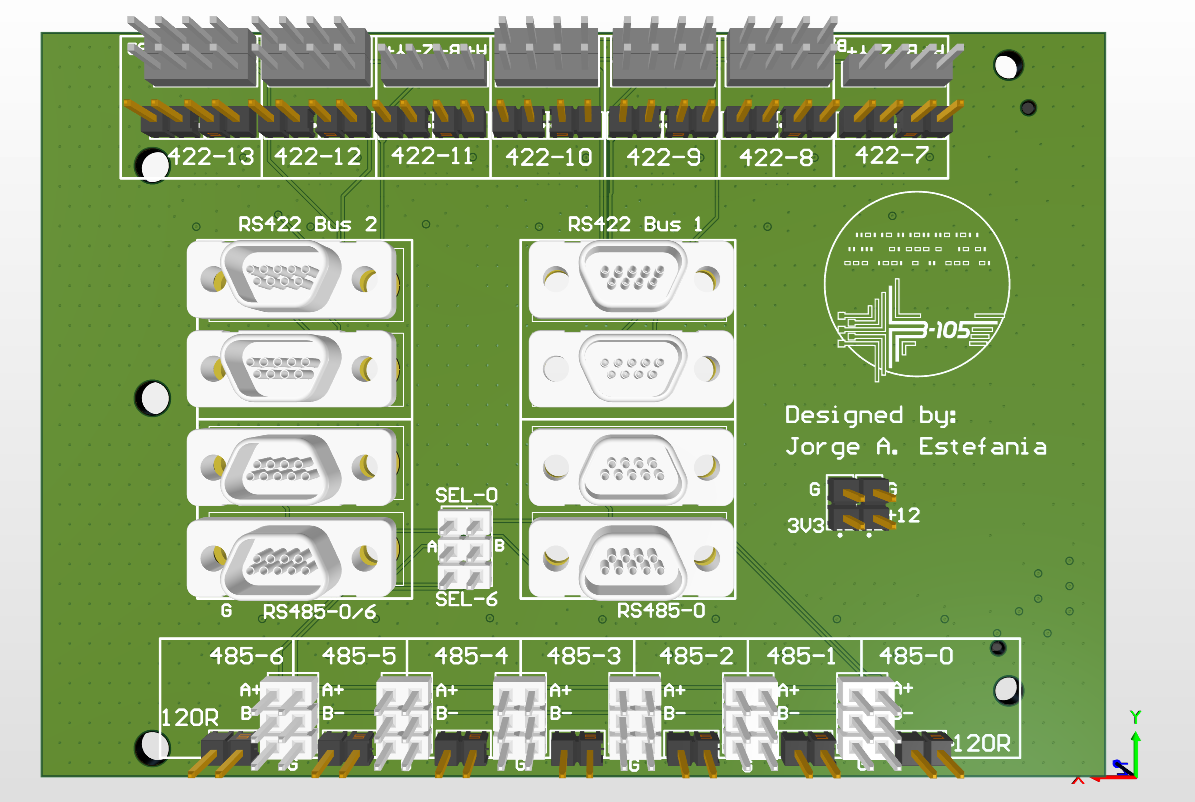
\includegraphics[width=\textwidth]{IMG/pcbs/serial_3d_top.png}
        \caption{Cara de conectores.}
    \end{subfigure}
    \hfill
    \begin{subfigure}[t]{0.48\textwidth}
        \centering
        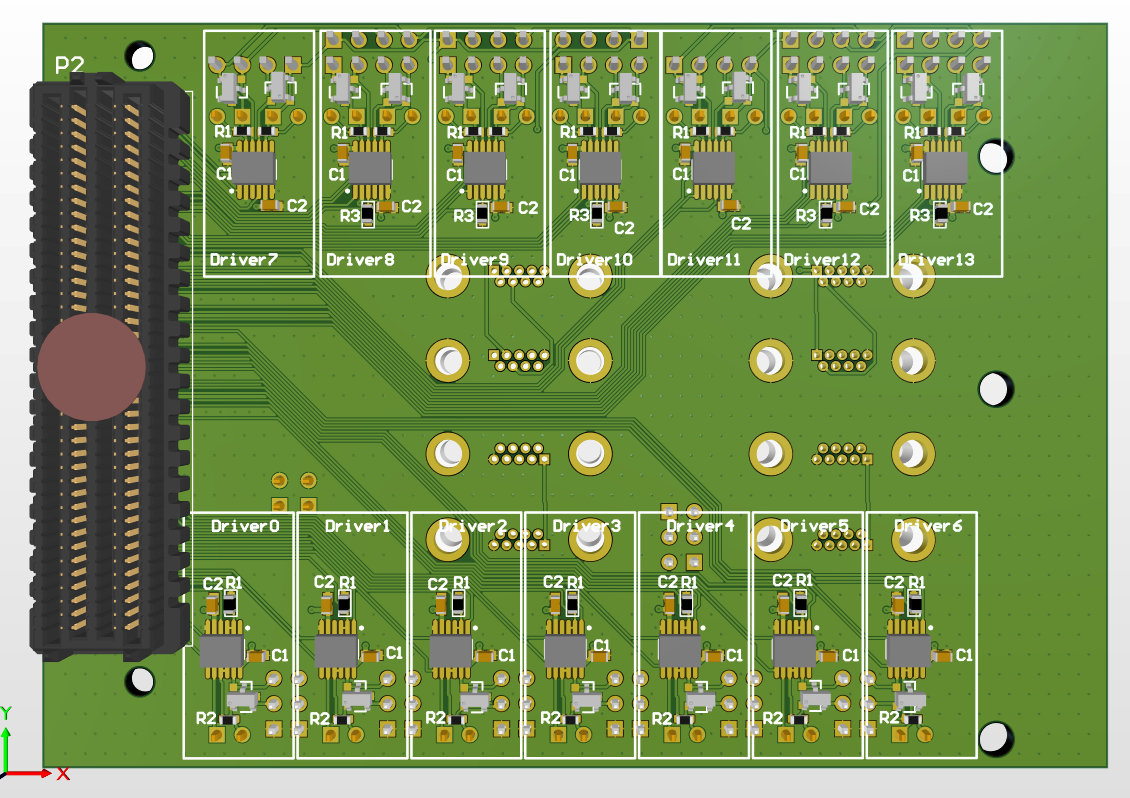
\includegraphics[width=\textwidth]{IMG/pcbs/serial_3d_bot.png}
        \caption{Cara de componentes.}
    \end{subfigure}
    \caption{Render 3D de la placa de comunicación serie.}
    \label{fig:serial_3d}
\end{figure}

\subsection{Topología RS485 con bus compartido configurable por \textit{jumper}}

La decisión de diseño más relevante de esta placa es el mecanismo de bus compartido RS485
sin necesidad de recablear. Cada driver RS485 tiene un conector Dupont de 3 pines
(A+, B$-$, GND) que actúa a la vez como punto de conexión hacia el exterior y como punto de
interconexión entre drivers adyacentes. Colocando un \textit{jumper} entre dos conectores
consecutivos, las líneas A y B de ambos drivers quedan físicamente unidas, formando un
segmento de bus RS485 compartido. Retirando el \textit{jumper}, el driver queda independiente y
puede conectarse a un periférico externo de forma individual.

Este mecanismo permite configurar por hardware cualquier partición de los 7 drivers RS485
en uno o varios buses, sin modificar el firmware ni el cableado exterior.

\subsection{Selector de conector Micro-D para RS485}

Los conectores de mayor densidad (Micro-D) de la placa son compartidos entre el Driver 0 y
el Driver 6 mediante un \textit{jumper} de selección de hardware. Dependiendo de la posición del
\textit{jumper}, los conectores Micro-D quedan asignados a uno u otro driver. Esto permite usar
un único tipo de conector con cableado de satélite, sin duplicar el número de conectores en
la placa.

\subsection{Topología RS422 maestro/esclavo configurable por \textit{jumper}}

Para RS422, cada driver \textit{slave} dispone de un conector con las líneas TX cruzadas a RX
(TX-Y+/TX-Z$-$ conectadas a RX del bus). Esta disposición replica la conexión estándar punto a
punto RS422, donde el receptor del esclavo escucha las transmisiones del \textit{master}. Al
igual que en RS485, un \textit{jumper} determina si el driver se une al bus común o permanece
independiente.

\subsection{Alimentación}

La placa se alimenta íntegramente del conector FMC, que suministra los carriles de 12~V, 3,3~V y
VADJ a 1,8~V. Los transceptores LTC2865 operan con la etapa de bus a 3,3~V (\texttt{VCC}) y la
interfaz lógica a 1,8~V (\texttt{VL}). A diferencia de las placas CDHS y AOCS, que generan con un
convertidor DC/DC los 5~V de su etapa de potencia, esta placa no necesita ninguna etapa de
conversión. Todos los carriles llegan directamente del FMC. Sendos conectores
de dos pines dan acceso externo a los carriles de 12~V y 3,3~V.

El mapa completo de señales entre esta placa y el conector FMC se encuentra en el
apartado~\ref{anxC:mapa_serial} del Anexo~\ref{anx:rtl}. El esquemático completo (12 hojas, PDF) y la BOM están disponibles en
\texttt{tfm/00\_docs/pcbs/serial/} del repositorio del proyecto.

% ----- CDHS -----
\section{Diseño de la placa CDHS}

La placa LINCE3 CDHS BreakoutBox es una tarjeta de interconexión entre la ZCU102
(conectada por FMC) y los periféricos del subsistema de gestión de datos y calentadores del
satélite. Sus especificaciones fueron definidas por Indra: 6 conectores D-Sub-9 (J1--J6),
interfaces CAN redundante, tres canales RS422/RS485, cuatro líneas PWM para calentadores
y un ADC para termistores. El esquemático se organizó en un bloque jerárquico por
subsistema, con el reparto que recoge la figura~\ref{fig:cdhs_top}. El resultado físico del
diseño se aprecia en el render de la figura~\ref{fig:cdhs_3d}.

\begin{figure}[htbp]
    \centering
    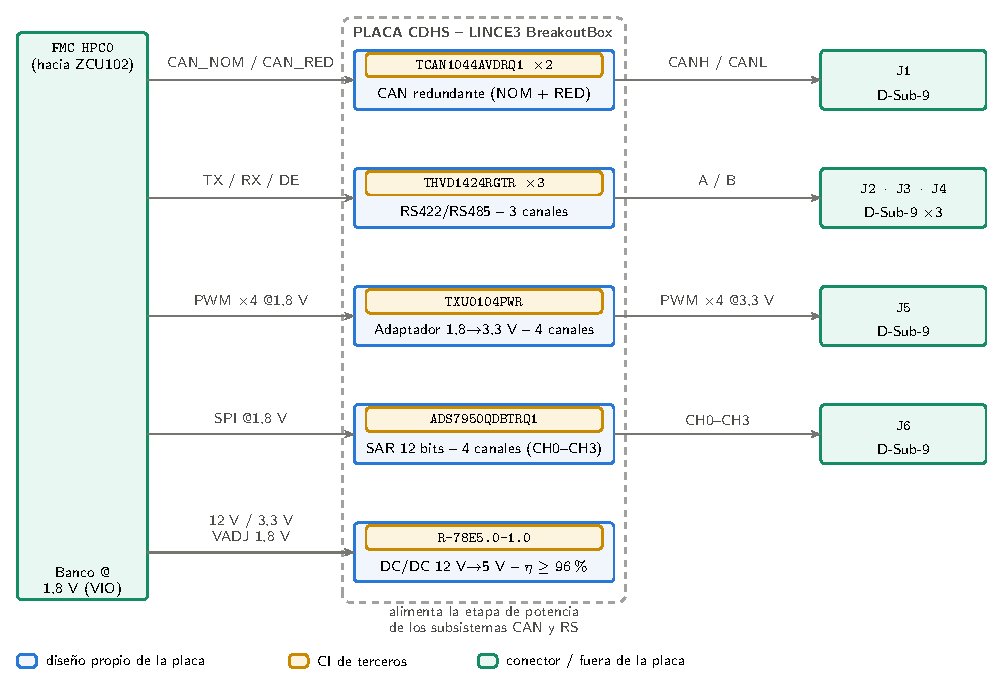
\includegraphics[width=\textwidth]{IMG/Desarrollo/diagrama_bloques_cdhs.pdf}
    \caption{Diagrama de bloques de la placa CDHS.}
    \label{fig:cdhs_top}
\end{figure}

\begin{figure}[htbp]
    \centering
    \begin{subfigure}[t]{0.48\textwidth}
        \centering
        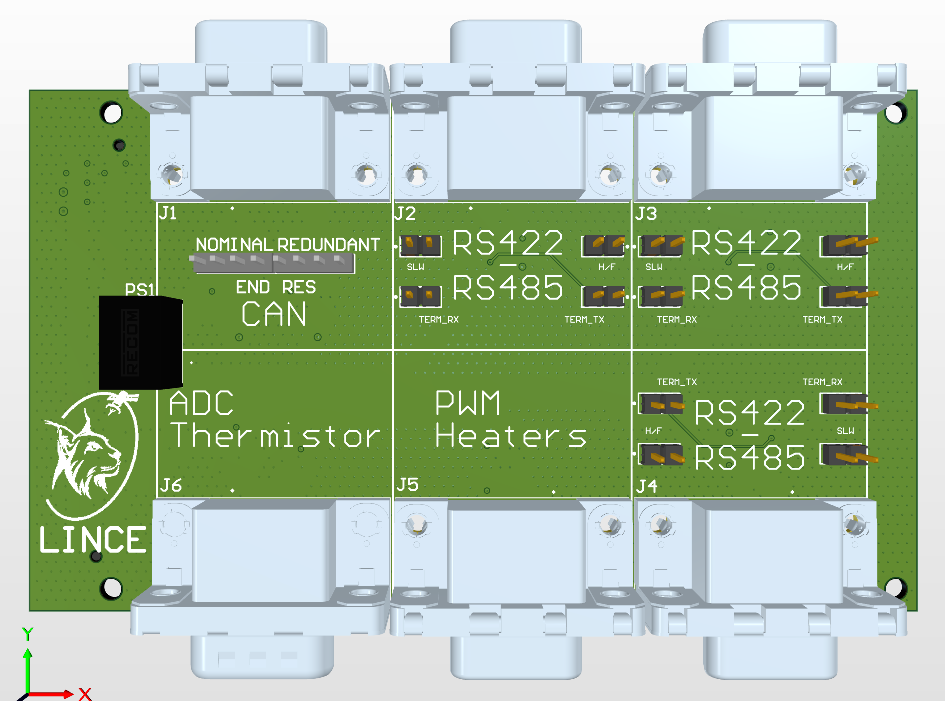
\includegraphics[width=\textwidth]{IMG/pcbs/cdhs_3d_top.png}
        \caption{Cara de conectores.}
    \end{subfigure}
    \hfill
    \begin{subfigure}[t]{0.48\textwidth}
        \centering
        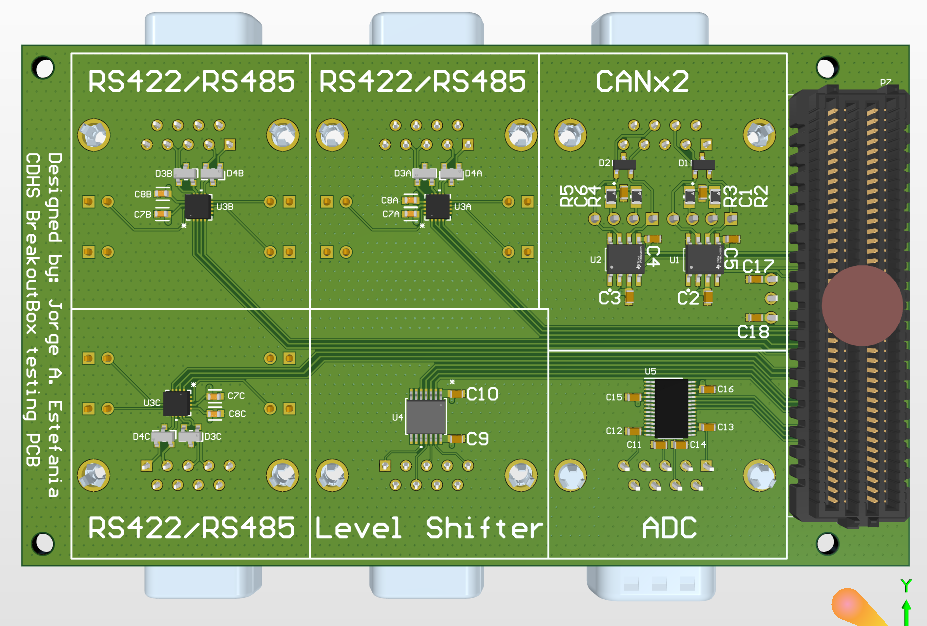
\includegraphics[width=\textwidth]{IMG/pcbs/cdhs_3d_bot.png}
        \caption{Cara de componentes.}
    \end{subfigure}
    \caption{Render 3D de la placa CDHS.}
    \label{fig:cdhs_3d}
\end{figure}

\subsection{Nivel de tensión y selección de componentes}

Como en las otras dos tarjetas, todos los bancos de pines del conector FMC HPC utilizados por esta
placa operan a 1,8~V. Los componentes se seleccionaron con \textit{VIO} nativo a ese nivel, para
evitar etapas de adaptación en la cadena de señal. Las implicaciones de esta restricción, y el
motivo por el que obligó a descartar los componentes con herencia de vuelo, se discuten en la
sección~\ref{sec:seleccion_componentes}. Los subsistemas que siguen aplican ese criterio, y las
excepciones (las señales de PWM, que sí requieren adaptación de nivel) se señalan donde
corresponde.

\subsection{Subsistema CAN}

El bus CAN implementa topología redundante con dos instancias independientes: CAN
Nominal (CAN\_NOM) y CAN Redundante (CAN\_RED). La elección del transceptor y de la terminación
parte del estudio de Diego Ramos para la plataforma CAN de LINCE~\cite{ramos2026can}. Se seleccionó el transceptor
\textbf{TCAN1044AVDRQ1} de Texas Instruments por su compatibilidad nativa con VIO de 1,8~V,
grado automotriz y baja corriente en modo \textit{standby}. Ambos canales convergen en el
conector J1.

Las resistencias de terminación siguen el esquema \textit{split termination} recomendado en las
notas de aplicación del estándar CAN (ISO 11898-2). En lugar de una única resistencia de
120~$\Omega$ entre CANH y CANL, se emplean \textbf{dos resistencias de 60~$\Omega$ en serie} con un
\textbf{condensador de 4,7~nF} conectado desde el punto medio al plano de masa. Cada una de
las dos resistencias de 60~$\Omega$ está controlada por un \textit{jumper} independiente, lo que
permite habilitar o deshabilitar la terminación sin modificar el circuito. La resistencia
equivalente sigue siendo 120~$\Omega$ cuando ambos \textit{jumpers} están colocados. El
condensador de derivación crea un camino de baja impedancia para las interferencias de
modo común de alta frecuencia hacia masa, lo que mejora el comportamiento EMC del bus.

Las líneas CANH y CANL de cada canal incorporan diodos de protección ESD
\textbf{ESDCAN24-2BLY}, específicamente diseñados para buses CAN. Clampean los transitorios
por encima de su tensión de ruptura sin introducir una capacitancia parásita significativa. La
figura~\ref{fig:cdhs_can} recoge el circuito completo de los dos canales.

\begin{figure}[htbp]
    \centering
    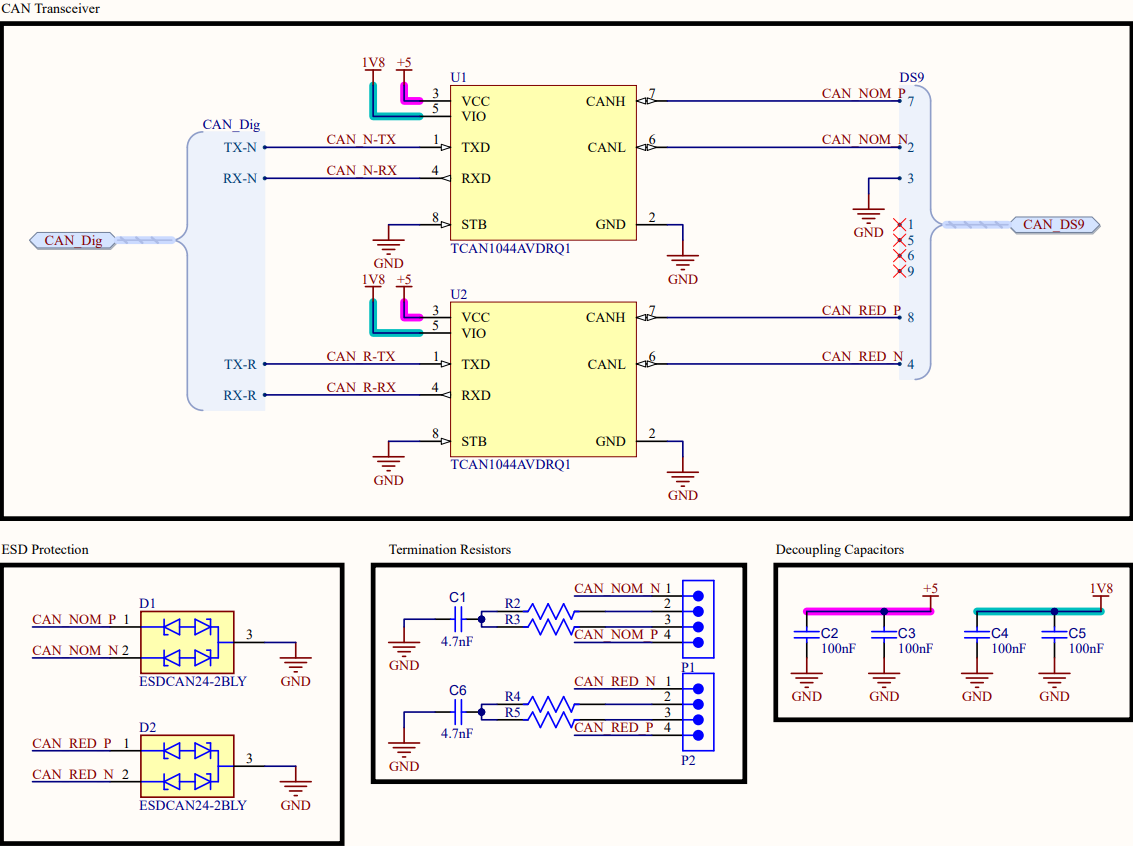
\includegraphics[width=\textwidth]{IMG/Esquematicos/CDHS_CAN.png}
    \caption{Subsistema CAN de la placa CDHS.}
    \label{fig:cdhs_can}
\end{figure}

\subsection{Subsistema RS422/RS485}

Se disponen tres canales serie idénticos e independientes (RS1, RS2, RS3), cada uno con el
transceptor \textbf{THVD1424RGTR}. Este integrado, sugerido dentro del proyecto LINCE con
posterioridad al diseño de la placa de comunicación serie propia, mejora al LTC2865 empleado en
aquella. Además de
soportar VIO de 1,8~V, incorpora resistencias de terminación internas conmutables y permite
seleccionar entre modo \textit{half-duplex} y \textit{full-duplex} sin cambiar el hardware. Por
estas ventajas se adoptó para las dos tarjetas oficiales. La configuración se expone mediante
\textit{jumpers} físicos de 2 pines: \textbf{H/F} (conmuta entre \textit{half-duplex} y \textit{full-duplex}), \textbf{SLR}
(habilita control de \textit{slew rate}), \textbf{TERM\_TX / TERM\_RX} (conectan las resistencias de
terminación internas). Los tres canales salen por los conectores J2, J3 y J4.

Tanto las líneas RX como las TX de cada canal llevan un par de diodos TVS
\textbf{SM712-02HTG} conectados entre las líneas diferenciales y el plano de masa.

\paragraph{Cortocircuito DE--RE.}
El THVD1424 expone dos pines de control independientes: \textbf{DE} (\textit{Driver Enable}, activo en
alto) habilita el transmisor, y \textbf{RE} (\textit{Receiver Enable}, activo en bajo) habilita el receptor.
En el esquemático, ambos pines están conectados a la misma señal de control procedente del
MPSoC. Una única línea digital controla así, de forma complementaria, transmisor y receptor
(tabla~\ref{tab:de_re}).

\begin{table}[H]
    \centering
    \begin{tabular}{ccc}
        \hline
        \textbf{Señal DE/RE} & \textbf{Transmisor (DE)} & \textbf{Receptor (RE activo bajo)} \\
        \hline
        1 (alto) & Habilitado & Deshabilitado \\
        0 (bajo) & Deshabilitado & Habilitado \\
        \hline
    \end{tabular}
    \caption{Control complementario DE/RE en el THVD1424.}
    \label{tab:de_re}
\end{table}

Esta decisión responde a dos motivos. Por un lado, el equipo de Indra comunicó que en la
arquitectura del satélite los esclavos solo transmiten bajo demanda del OBC. Por ello, no
existe un escenario real en el que un nodo deba transmitir y recibir simultáneamente. Por
otro lado, en modo \textit{half-duplex} las líneas TX y RX comparten físicamente el mismo par
diferencial A/B. Si el receptor permaneciera activo durante la transmisión, el nodo escucharía
su propio eco. El circuito completo de un canal, con esa conexión y los cuatro \textit{jumpers}
de configuración, es el de la figura~\ref{fig:cdhs_rs}.

\begin{figure}[htbp]
    \centering
    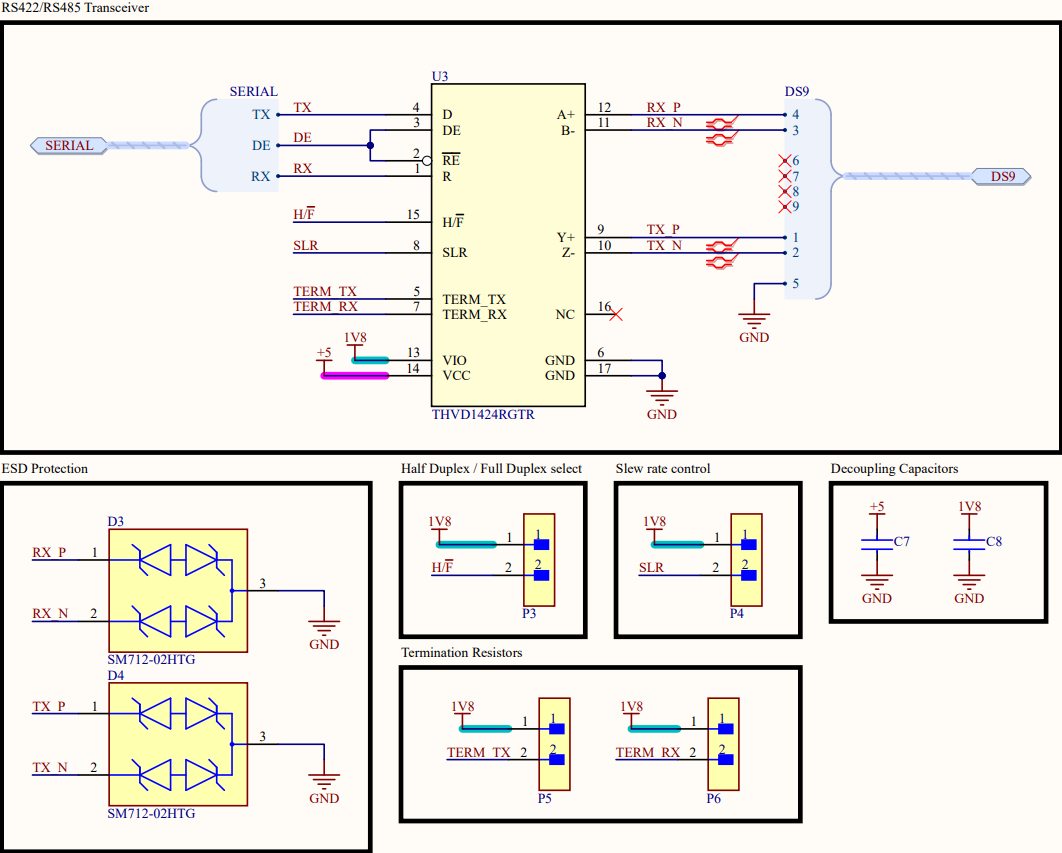
\includegraphics[width=\textwidth]{IMG/Esquematicos/CDHS_RS.png}
    \caption{Canal RS de la placa CDHS con el THVD1424RGTR.}
    \label{fig:cdhs_rs}
\end{figure}

\subsection{Subsistema PWM (calentadores)}

Cuatro señales PWM de 1,8~V procedentes del FMC se elevan a 3,3~V mediante el adaptador
de niveles \textbf{TXU0104PWR} para excitar los circuitos de control de calentadores externos.
Las cuatro líneas adaptadas salen por J5.

Para la validación de esta interfaz se diseñó un bloque VHDL autónomo,
\texttt{PWMx4\_\allowbreak auto\_test}, sintetizado en la PL junto al resto del diseño de Vivado. El bloque
genera cuatro señales PWM independientes con \textit{duty cycle} del 50\,\% a partir del reloj de
100~MHz de la FPGA: canal 0 a 10~kHz, canal 1 a 5~kHz, canal 2 a 1~kHz y canal 3 a
100~Hz. Al ser completamente autónomo no requiere ningún driver ni intervención del PS, lo
que permitió verificar el subsistema PWM de la placa con el mismo BOOT.BIN utilizado para
las pruebas serie.

\subsection{Subsistema ADC (termistores)}

Cuatro entradas analógicas de termistores (CH0--CH3) se digitalizan con el ADC SAR de
12 bits \textbf{ADS7950QDBTRQ1}, comunicado al procesador por SPI a 1,8~V. La circuitería
analógica opera a 3,3~V. Ambos carriles (+VBD a 1,8~V y +VA a 3,3~V) son independientes,
para evitar acoplos entre el dominio digital y el analógico~\cite{ti2018ads7950}. Los
termistores se conectan por J6.

\subsection{Alimentación}

El conector FMC suministra 12~V, 3,3~V y el carril VADJ a 1,8~V. El convertidor conmutado
\textbf{R-78E5.0-1.0} genera los 5~V necesarios para la etapa de potencia de los transceptores
RS y CAN a partir de los 12~V del FMC. Se eligió este módulo DC/DC por su integración en
un \textit{footprint} reducido de 3 pines (equivalente a un regulador lineal) y su eficiencia
$\geq$~96\,\%, evitando la disipación térmica que tendría un LDO con ese diferencial de tensión.

\subsection{Conectores externos}

Los seis puertos D-Sub-9 (J1--J6) son de tipo macho o hembra según la convención de uso.
Los escudos metálicos de todos los conectores están conectados al plano de GND para
mantener la continuidad de apantallamiento EMI con los cables blindados.

El mapa completo de señales entre la placa CDHS y el conector FMC se encuentra en el
apartado~\ref{anxC:mapa_cdhs} del Anexo~\ref{anx:rtl}. El esquemático (PDF) y la BOM están disponibles en
\texttt{tfm/00\_docs/pcbs/cdhs/}.

% ----- AOCS -----
\section{Diseño de la placa AOCS} \label{sec:diseno_aocs}

La placa LINCE3 AOCS BreakoutBox es la tarjeta de interconexión para el subsistema de
control de actitud y órbita del satélite. Al igual que la CDHS, conecta la ZCU102 mediante
FMC y expone las interfaces al exterior a través de 8 conectores D-Sub-9 (J1--J8). La
figura~\ref{fig:aocs_top} muestra cómo se reparten esas ocho salidas entre los distintos
subsistemas, y la figura~\ref{fig:aocs_3d} recoge el aspecto físico de la tarjeta.

Lo que se describe a continuación es la \textbf{revisión V2} del diseño, que es la versión
cerrada del esquemático. Las dos unidades fabricadas y toda la validación
recogida en la sección~\ref{sec:validacion_aocs} corresponden a la \textbf{revisión anterior},
de cinco canales serie. La V2 no llegó a fabricarse. Las diferencias entre ambas
revisiones son cuatro: el desdoble del canal de J4 en dos, la separación de las líneas DE y RE,
la adición de puntos de prueba y la corrección de un error de conexión en el eje Z del bloque
de motores. Las tres primeras se detallan en el subsistema RS que sigue, y la cuarta en el de
MOT-PWM.

\begin{figure}[htbp]
    \centering
    
\includegraphics[width=0.92\textwidth]{IMG/Esquematicos/AOCS.png}
    \caption{Hoja de nivel superior del esquemático de la placa AOCS.}
    \label{fig:aocs_top}
\end{figure}

\begin{figure}[htbp]
    \centering
    \begin{subfigure}[t]{0.48\textwidth}
        \centering
        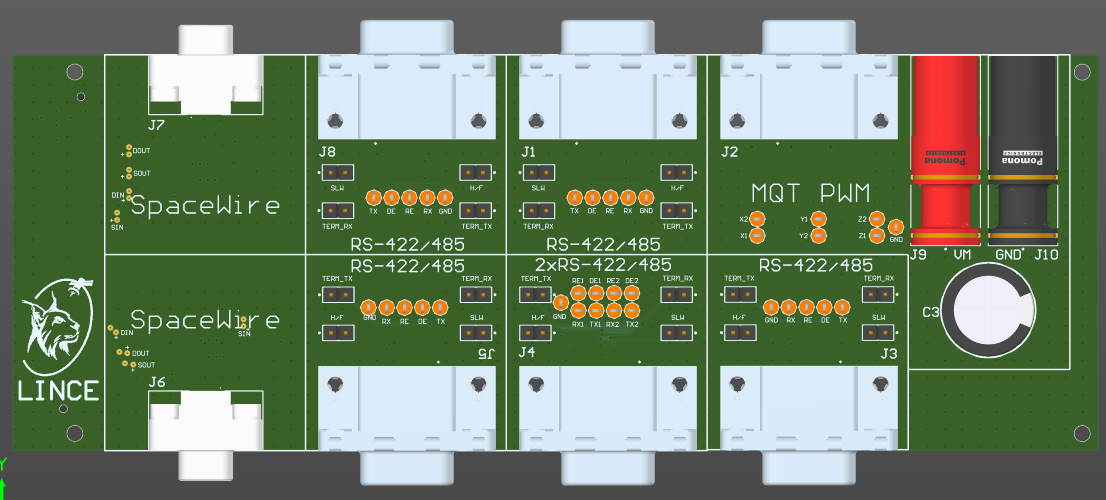
\includegraphics[width=\textwidth]{IMG/pcbs/aocs_3d_top.png}
        \caption{Cara de conectores.}
    \end{subfigure}
    \hfill
    \begin{subfigure}[t]{0.48\textwidth}
        \centering
        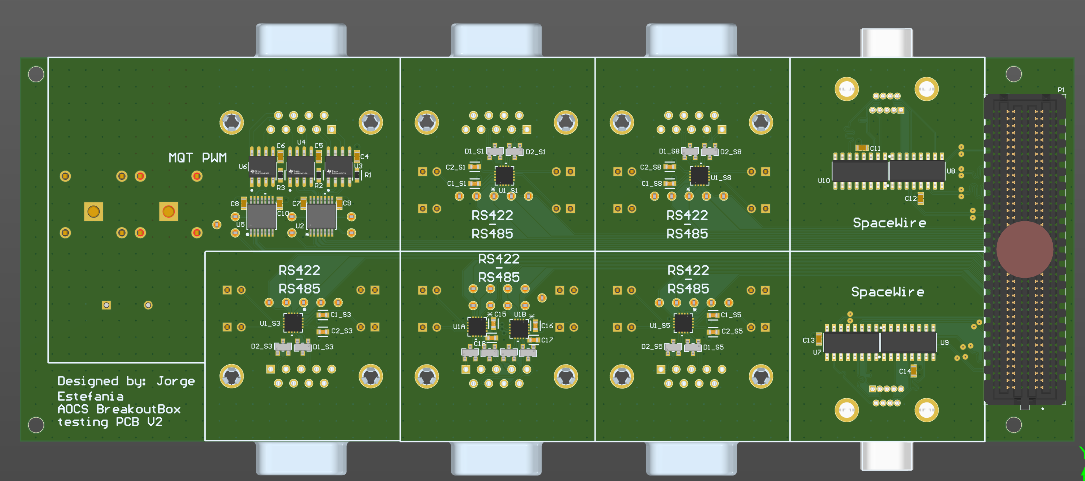
\includegraphics[width=\textwidth]{IMG/pcbs/aocs_3d_bot.png}
        \caption{Cara de componentes.}
    \end{subfigure}
    \caption{Render 3D de la revisión V2 de la placa AOCS.}
    \label{fig:aocs_3d}
\end{figure}

\subsection{Subsistema RS422/RS485}

La placa incorpora \textbf{seis canales serie} (RS1, RS3, RS41, RS42, RS5 y RS8) con el mismo
transceptor THVD1424RGTR descrito en la sección de la placa CDHS. Usa los mismos \textit{jumpers}
de configuración H/F, SLR y terminación. Los canales RS41 y RS42 comparten el conector J4: la
hoja \texttt{RSx2} monta los dos transceptores de ese conector. Los seis canales salen así por
cinco D-Sub-9 (J1, J3, J4$\times$2, J5 y J8). Frente a la revisión anterior, de cinco canales, el
desdoble permite ejercitar un par \textit{master/slave} completo sobre un único conector.

Respecto al diseño de la CDHS hay una diferencia de fondo: en esta placa las líneas
\textbf{DE y RE llegan por separado} desde el MPSoC, en lugar de cortocircuitadas. Cada canal
consume así cuatro señales digitales del FMC (TX, RX, DE y RE) en vez de tres. El motivo es que
el cortocircuito DE--RE fija el comportamiento en el cobre: obliga a que el receptor esté
siempre en el estado complementario del transmisor, que es lo que la arquitectura del satélite
necesita. Sin embargo, impide comprobar en banco cualquier otra combinación. Con las dos líneas
independientes, el firmware puede seguir imponiendo el comportamiento complementario por
software. Además, permite habilitar receptor y transmisor a la vez para observar el eco propio en
\textit{half-duplex}, o dejar ambos deshabilitados para verificar que la línea queda en alta
impedancia.

\paragraph{Puntos de prueba.}
La revisión V2 añade \textbf{puntos de prueba} en las cuatro líneas lógicas de cada canal
(TX, DE, RE y RX), más una toma de masa por bloque. Son accesibles desde la cara de conectores,
junto a los \textit{jumpers} (figura~\ref{fig:aocs_3d}). El bloque de PWM de motores lleva los
suyos sobre los seis pares X1/X2, Y1/Y2 y Z1/Z2, también con masa propia. La razón es la
depuración. Los caracteres corruptos que motivaron los estados \texttt{PreDE} y \texttt{PostDE}
del transmisor se diagnosticaron pinchando el osciloscopio en el lado lógico del transceptor. En
la revisión anterior, esas líneas solo eran accesibles en las patas del encapsulado. Una toma de
masa contigua a cada grupo de señales es parte del mismo objetivo: el lazo de masa de la punta es
lo que limita la fidelidad de la medida en flancos de varios megabaudios.

\subsection{Subsistema SpaceWire}

Se implementan dos enlaces SpaceWire \textit{full-duplex} independientes (SPW1 y SPW2) mediante
señalización diferencial LVDS. El estándar SpaceWire opera directamente a niveles LVDS
compatibles con los bancos del FMC. Ambos enlaces son idénticos y atraviesan \textbf{repetidores
LVDS DS90CP22M}, como muestra la figura~\ref{fig:aocs_spw}. Cada enlace lleva dos repetidores de
dos canales: uno para el sentido entrante (los pares DIN y SIN) y otro para el saliente (SOUT y
DOUT), lo que suma cuatro integrados en la placa. El repetidor reacondiciona los flancos y
aísla el tramo de cobre de la tarjeta del cable externo, que es donde el enlace se degrada. Su
coste es un retardo de propagación fijo, irrelevante frente a la temporización de SpaceWire. La
simetría entre los dos enlaces permite además atribuir al cableado, y no a la placa, cualquier
diferencia que se observe entre ellos en banco. Los pares
diferenciales (cuatro por enlace: DIN, SIN, SOUT y DOUT) se han trazado en la PCB con
técnicas de igualación de longitud (\textit{length matching}), para minimizar el \textit{skew}
entre el par de datos y el par de \textit{strobe}. También se ha controlado su impedancia
característica, de 100~$\Omega$ diferencial.

\begin{figure}[htbp]
    \centering
    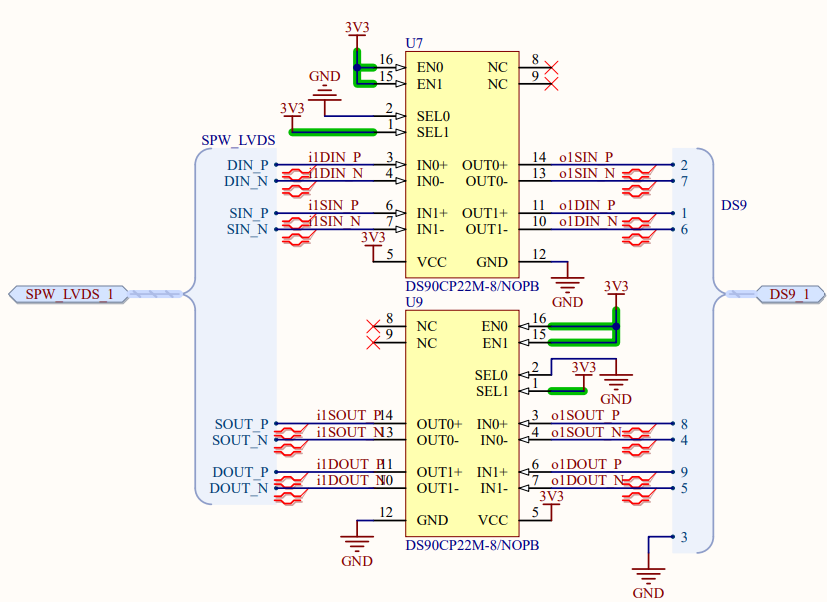
\includegraphics[width=0.88\textwidth]{IMG/Esquematicos/AOCS_SPW_1.png}
    \caption{Subsistema SpaceWire de la placa AOCS.}
    \label{fig:aocs_spw}
\end{figure}

\subsection{Subsistema de control de motores (MOT-PWM)}

Seis señales PWM de 1,8~V procedentes del FMC se elevan al nivel de tensión requerido por
los puentes en H externos mediante un adaptador de niveles. Las señales se agrupan en tres
pares (X, Y, Z para los tres ejes del satélite), con dos líneas por eje para controlar la
dirección de giro del motor. Salen por J2. La alimentación de potencia de los motores se
conecta mediante dos bornes banana independientes de la alimentación de la placa.

Los seis pares se reparten entre dos adaptadores TXU0104PWR de cuatro canales: U2 lleva los
ejes X e Y, y U5 el eje Z, que ocupa solo dos de sus cuatro canales.

\paragraph{Corrección de la revisión V2: el eje Z.}
La revisión fabricada tenía un \textbf{error de conexión en el eje Z} que la V2 corrige. En
U5, las señales \texttt{PWM\_Z\_1} y \texttt{PWM\_Z\_2} entraban por A2 y A1, cuyas salidas
correspondientes eran B2Y y B1Y. Sin embargo, las entradas del puente en H de ese eje (U6) no
colgaban de B2Y y B1Y, sino de \textbf{B4Y y B3Y}, que eran las salidas de los dos canales no
utilizados. Esos dos canales tenían además sus entradas A4 y A3 \textbf{atadas a masa}, junto a
los pines NC del integrado. El resultado era que el eje Z quedaba fijo a nivel bajo en el
conector, por mucho que la PL generase la señal. Las dos líneas que la transportaban terminaban
en salidas del adaptador sin conectar, y las que llegaban al puente en H estaban permanentemente
a cero.

Ninguna comprobación automática detecta este fallo: el diseño es eléctricamente correcto y no
incumple ninguna regla de Altium. El comprobador de conectividad no ve nada anómalo, porque las
dos salidas sobrantes son terminaciones válidas y las entradas a masa son una conexión legítima.
Solo se manifiesta al medir el eje Z en el conector. La V2 reencamina las entradas de U6 a B2Y y
B1Y, que es donde salen efectivamente las señales del eje.

\subsection{Alimentación}

Misma arquitectura que la placa CDHS: 12~V del FMC, convertidor DC/DC para los 5~V de
potencia, y VADJ 1,8~V para los transceptores. La única diferencia es la etapa de potencia de
los motores, que no se alimenta del FMC: admite alimentación exterior a través de los dos
bornes banana, independiente del resto de la placa.

El mapa completo de señales entre la placa AOCS y el conector FMC se encuentra en el
apartado~\ref{anxC:mapa_aocs} del Anexo~\ref{anx:rtl}. Los esquemáticos (PDF) y la BOM están disponibles en
\texttt{tfm/00\_docs/pcbs/aocs/}. El fichero \texttt{LINCE3\_AOCS\_V2.pdf} es la revisión aquí
descrita, la única que refleja el estado final del diseño, y del que proceden todas las hojas de
esquemático reproducidas en esta sección. \texttt{LINCE3\_AOCS.pdf} es un volcado anterior que se
conserva por trazabilidad, pero está desactualizado incluso respecto a lo que se fabricó.

% ----- FABRICACIÓN -----
\section{Fabricación}

Una vez validados los esquemáticos y completado el rutado de las PCBs, se encargaron las
placas con \textit{stencil} a \textbf{PCBWay}, y los componentes a \textbf{Mouser} y \textbf{DigiKey} según
disponibilidad. El proceso de montaje en el laboratorio siguió los pasos habituales de
soldadura por reflujo SMD:

\begin{enumerate}
    \item \textbf{Aplicación de pasta de soldadura.} Se fijó la placa a la mesa con placas de
    idéntico grosor alrededor y cinta de pintor. Se colocó el \textit{stencil} alineado y se extendió
    la pasta con espátula.
    \item \textbf{Colocación de componentes.} Con pinzas de punta fina, se colocaron los
    componentes SMD sobre la pasta. Se montaron dos placas en paralelo para optimizar el
    tiempo de proceso.
    \item \textbf{Reflujo.} Las placas se introdujeron en el horno de reflujo del laboratorio
    seleccionando el perfil de temperatura adecuado para la pasta de soldadura utilizada.
\end{enumerate}

Las figuras~\ref{fig:cdhs_soldada} y~\ref{fig:aocs_soldada} muestran las placas CDHS y AOCS ya
montadas al salir del horno, que son las que se emplean en toda la campaña de validación
(sección~\ref{sec:validacion_cdhs} y siguientes).

\begin{figure}[htbp]
    \centering
    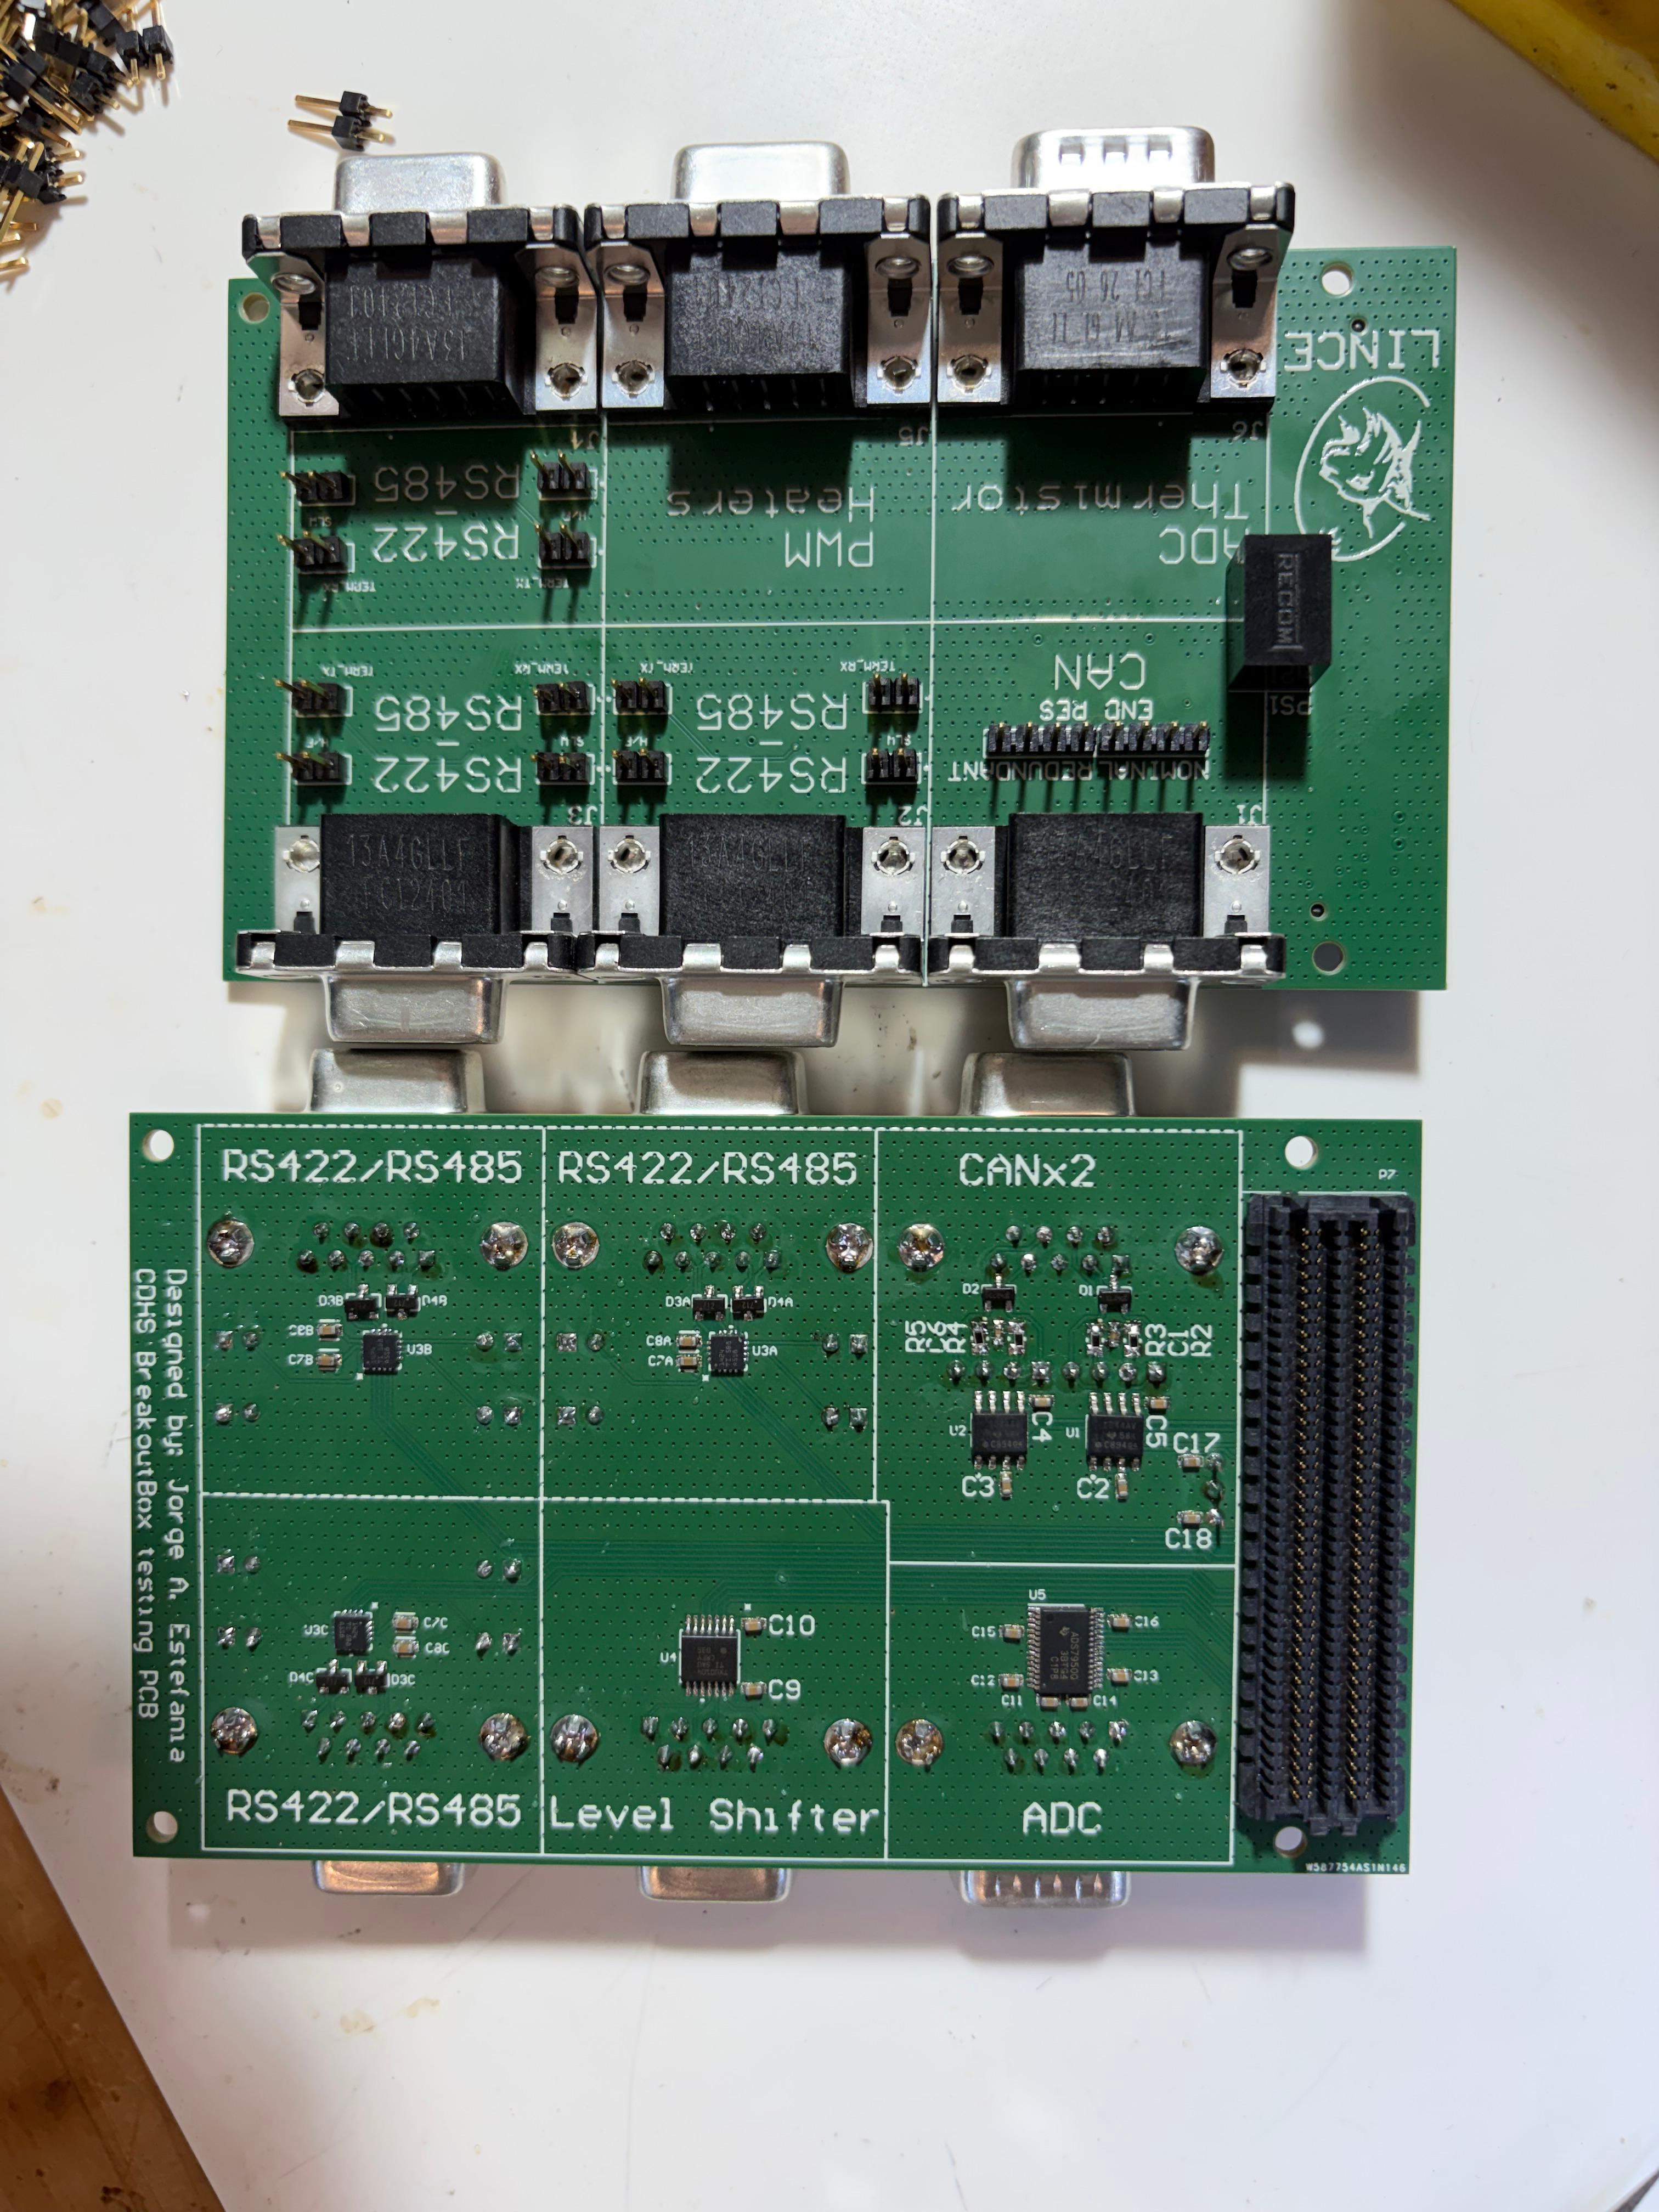
\includegraphics[width=0.62\textwidth]{IMG/cdhs_soldada.jpg}
    \caption{Placa CDHS tras el proceso de soldadura.}
    \label{fig:cdhs_soldada}
\end{figure}

\begin{figure}[htbp]
    \centering
    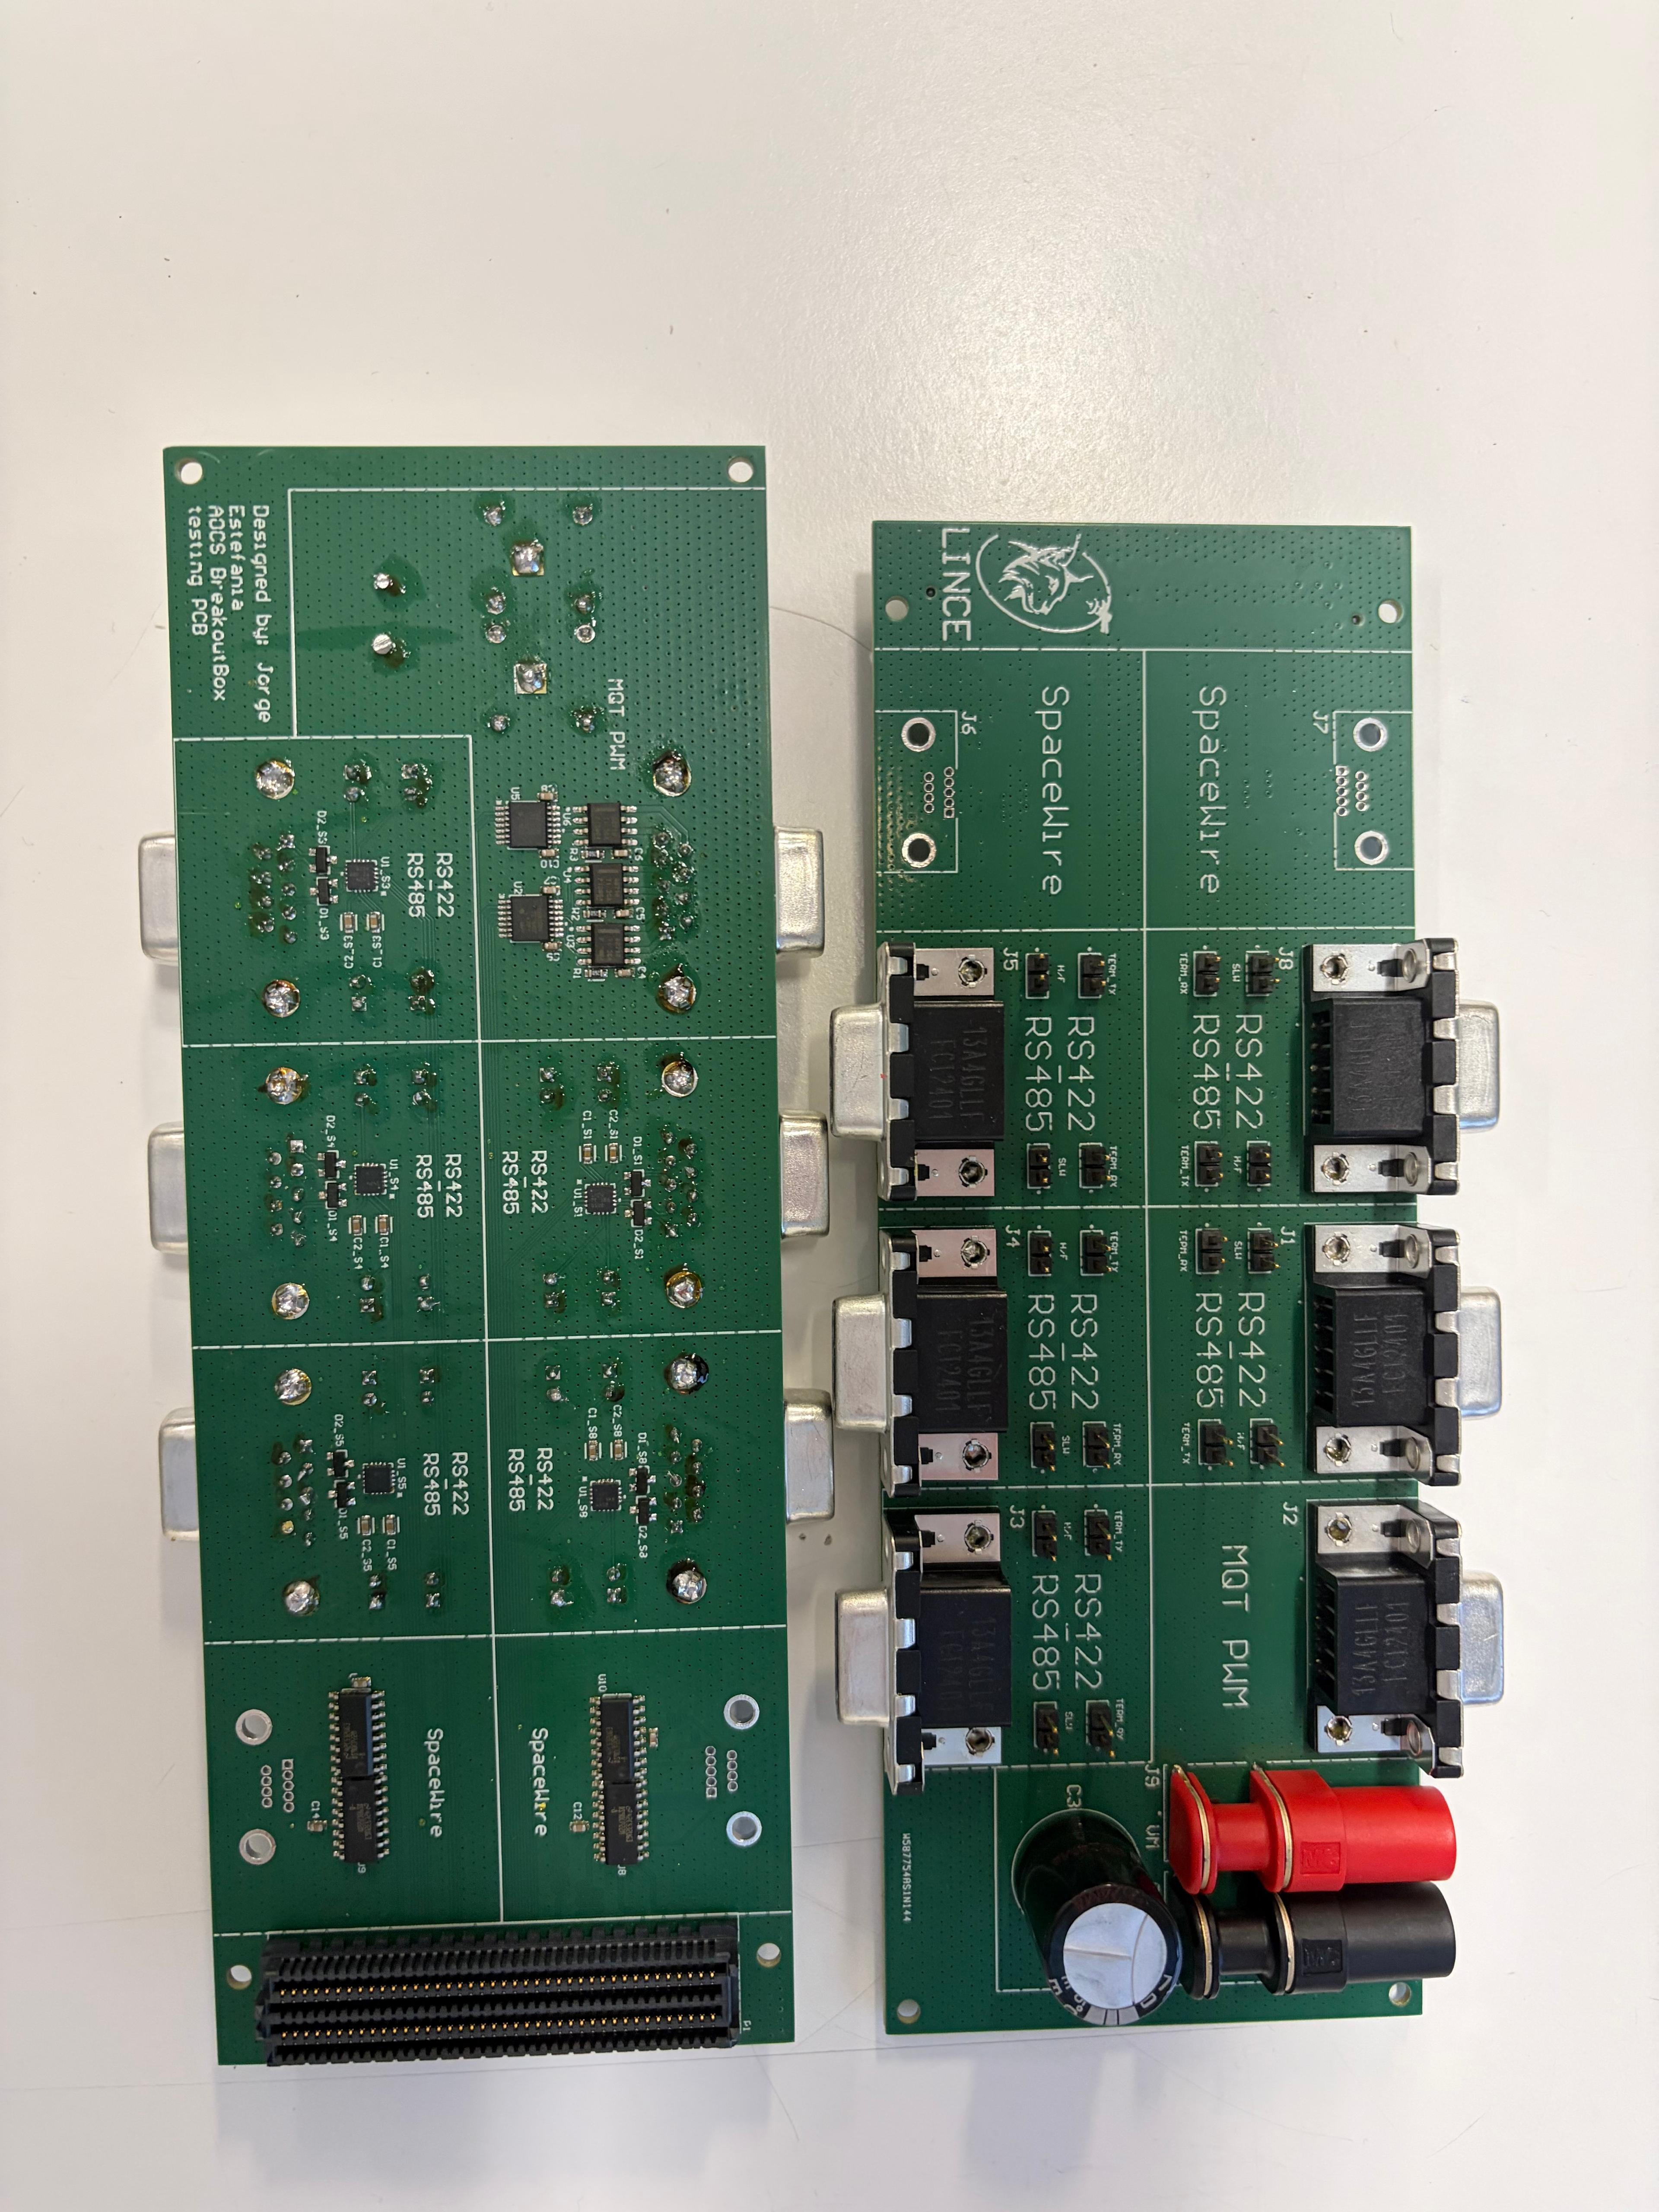
\includegraphics[width=0.62\textwidth]{IMG/aocs_soldada_caras.jpg}
    \caption{Placa AOCS tras el proceso de soldadura.}
    \label{fig:aocs_soldada}
\end{figure}

La placa de comunicación serie se montó por el mismo procedimiento. La figura~\ref{fig:serial_soldada}
muestra sus dos caras ya pobladas: los conectores D-Sub y los \textit{jumpers} de configuración
en el anverso, y los catorce transceptores LTC2865 en el reverso.

\begin{figure}[htbp]
    \centering
    \begin{subfigure}[t]{0.48\textwidth}
        \centering
        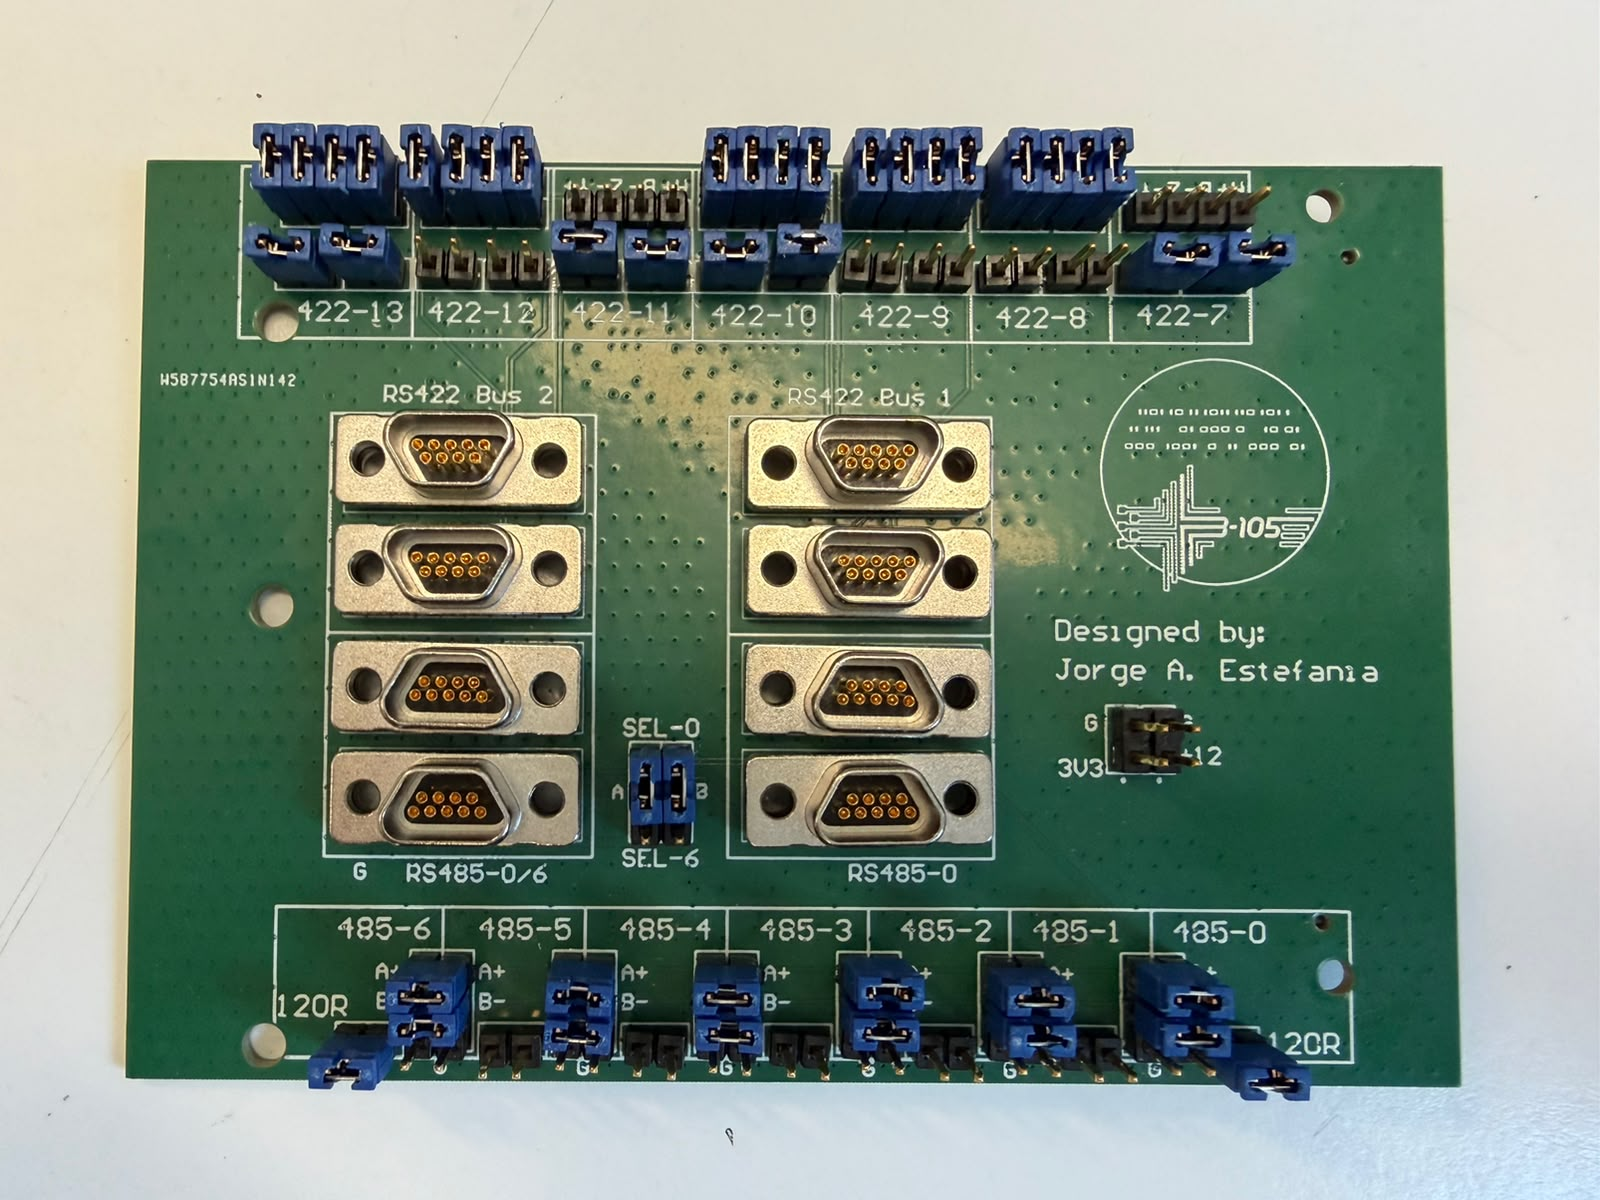
\includegraphics[width=\textwidth]{IMG/serial_pcb_jumpers.jpg}
        \caption{Cara de conectores.}
    \end{subfigure}
    \hfill
    \begin{subfigure}[t]{0.48\textwidth}
        \centering
        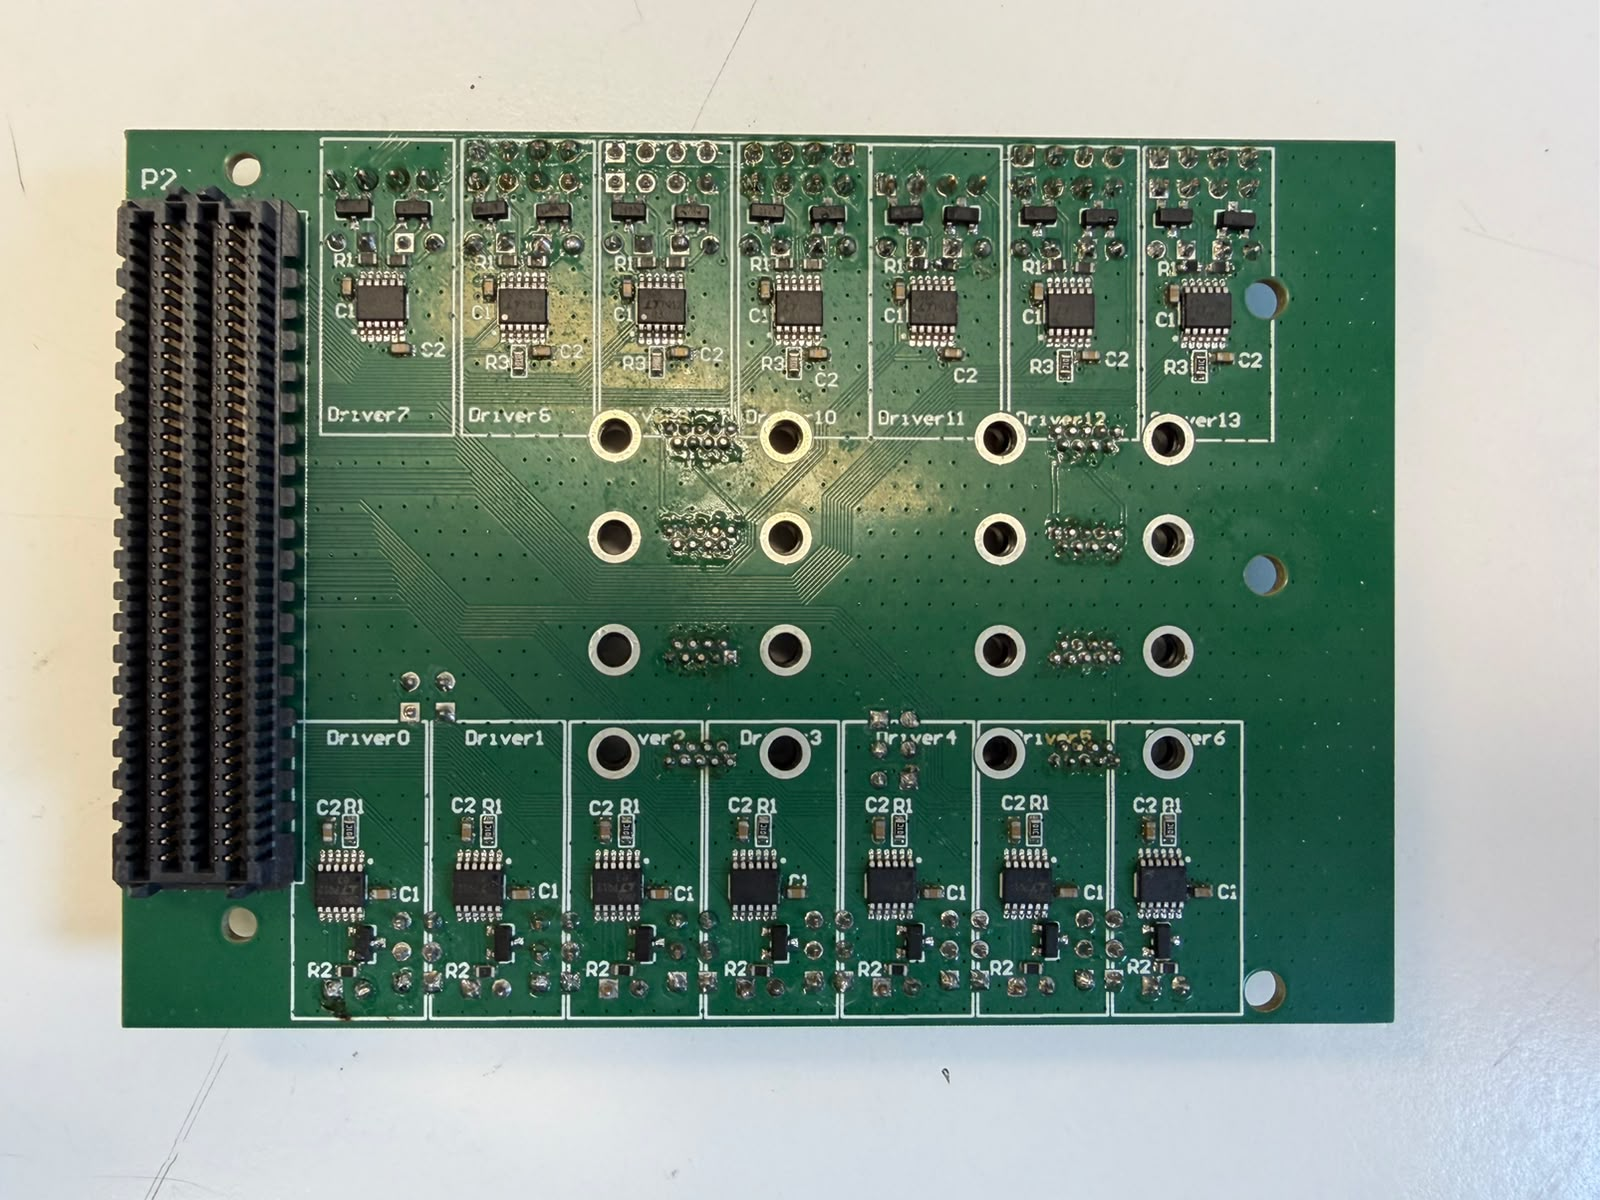
\includegraphics[width=\textwidth]{IMG/serial_pcb_top.jpg}
        \caption{Cara de componentes.}
    \end{subfigure}
    \caption{Placa de comunicación serie tras el proceso de soldadura.}
    \label{fig:serial_soldada}
\end{figure}
